\chapter{Methodology}
% Due by July 1, 2025
% Target: 25-30 pages
\label{chap:methodology}

\section{Introduction}
This chapter details the systematic methodology for developing and evaluating a system that leverages Large Language Models (LLMs) to convert extensive legal documents into attributed knowledge graphs (KGs) \parencite{RefWorks:RefID:102-hogan2021knowledge, RefWorks:RefID:120-fensel2020knowledge}. As established in Chapter 1, these KGs are intended to serve as a foundation for subsequent analysis of document completeness and consistency \parencite{RefWorks:RefID:10-zowghi2003interplay, RefWorks:RefID:29-umar2024advances}. The challenge of managing the complexity and scale of modern textual documents, particularly in legal codification, necessitates automated solutions \parencite{RefWorks:RefID:165-bhattacharya2019comparative}. Traditional manual review is often insufficient for ensuring comprehensive consistency in large, evolving document sets. This research posits that KGs, by providing structured representations of entities and their relationships, offer a viable approach to address these challenges \parencite{RefWorks:RefID:121-zhong2024comprehensive}.

The methodology herein is designed to be rigorous and reproducible. It outlines the overall research approach, system architecture, and data sources—specifically, Pennsylvania township laws. The chapter then details the critical hyperparameters governing the system, the experimental plan for their tuning, the software tools utilized, and the multi-faceted strategy for evaluating the quality of the generated KGs in the absence of a definitive ground truth. Finally, the inherent limitations of the chosen methods and relevant ethical considerations are examined, concluding with a restatement of the research questions and hypotheses this framework aims to address.

\section{Approach}
This research introduces Mnemosyne, a novel, multi-stage pipeline for transforming large, complex legislative documents into queryable Knowledge Graphs (KGs). Hereafter, this system will be referred to as Mnemosyne. By leveraging Large Language Models (LLMs) \parencite{RefWorks:RefID:107-benjira2025automated, RefWorks:RefID:162-lairgi2024knowledge}, our system is designed to facilitate automated analysis of legal texts for internal consistency and completeness. The architecture prioritizes two critical features: **usability**, requiring minimal specialized skill for operation, and **traceability**, ensuring every piece of information in the KG can be precisely linked to its source sentence. While developed using legal corpora, the modular design is generalizable to other domains characterized by large, structured documents \parencite{RefWorks:RefID:116-shaham2022scrolls}.

\subsection{Architectural Overview}
The system employs a modular pipeline that synthesizes established KG construction practices \parencite{RefWorks:RefID:118-ji2022survey} with a novel, two-tiered memory architecture adapted for the legal domain. This design manages the inherent complexity and context window limitations of modern LLMs \parencite{RefWorks:RefID:99-liu2025comprehensive} by building the KG iteratively. The data flows through a sequence of components, from initial document processing to advanced semantic enrichment. This modularity permits targeted optimization and evaluation at each stage. \Cref{fig:proposed_architecture} provides a high-level depiction of this data flow.

\begin{figure}[htbp]
    \centering
    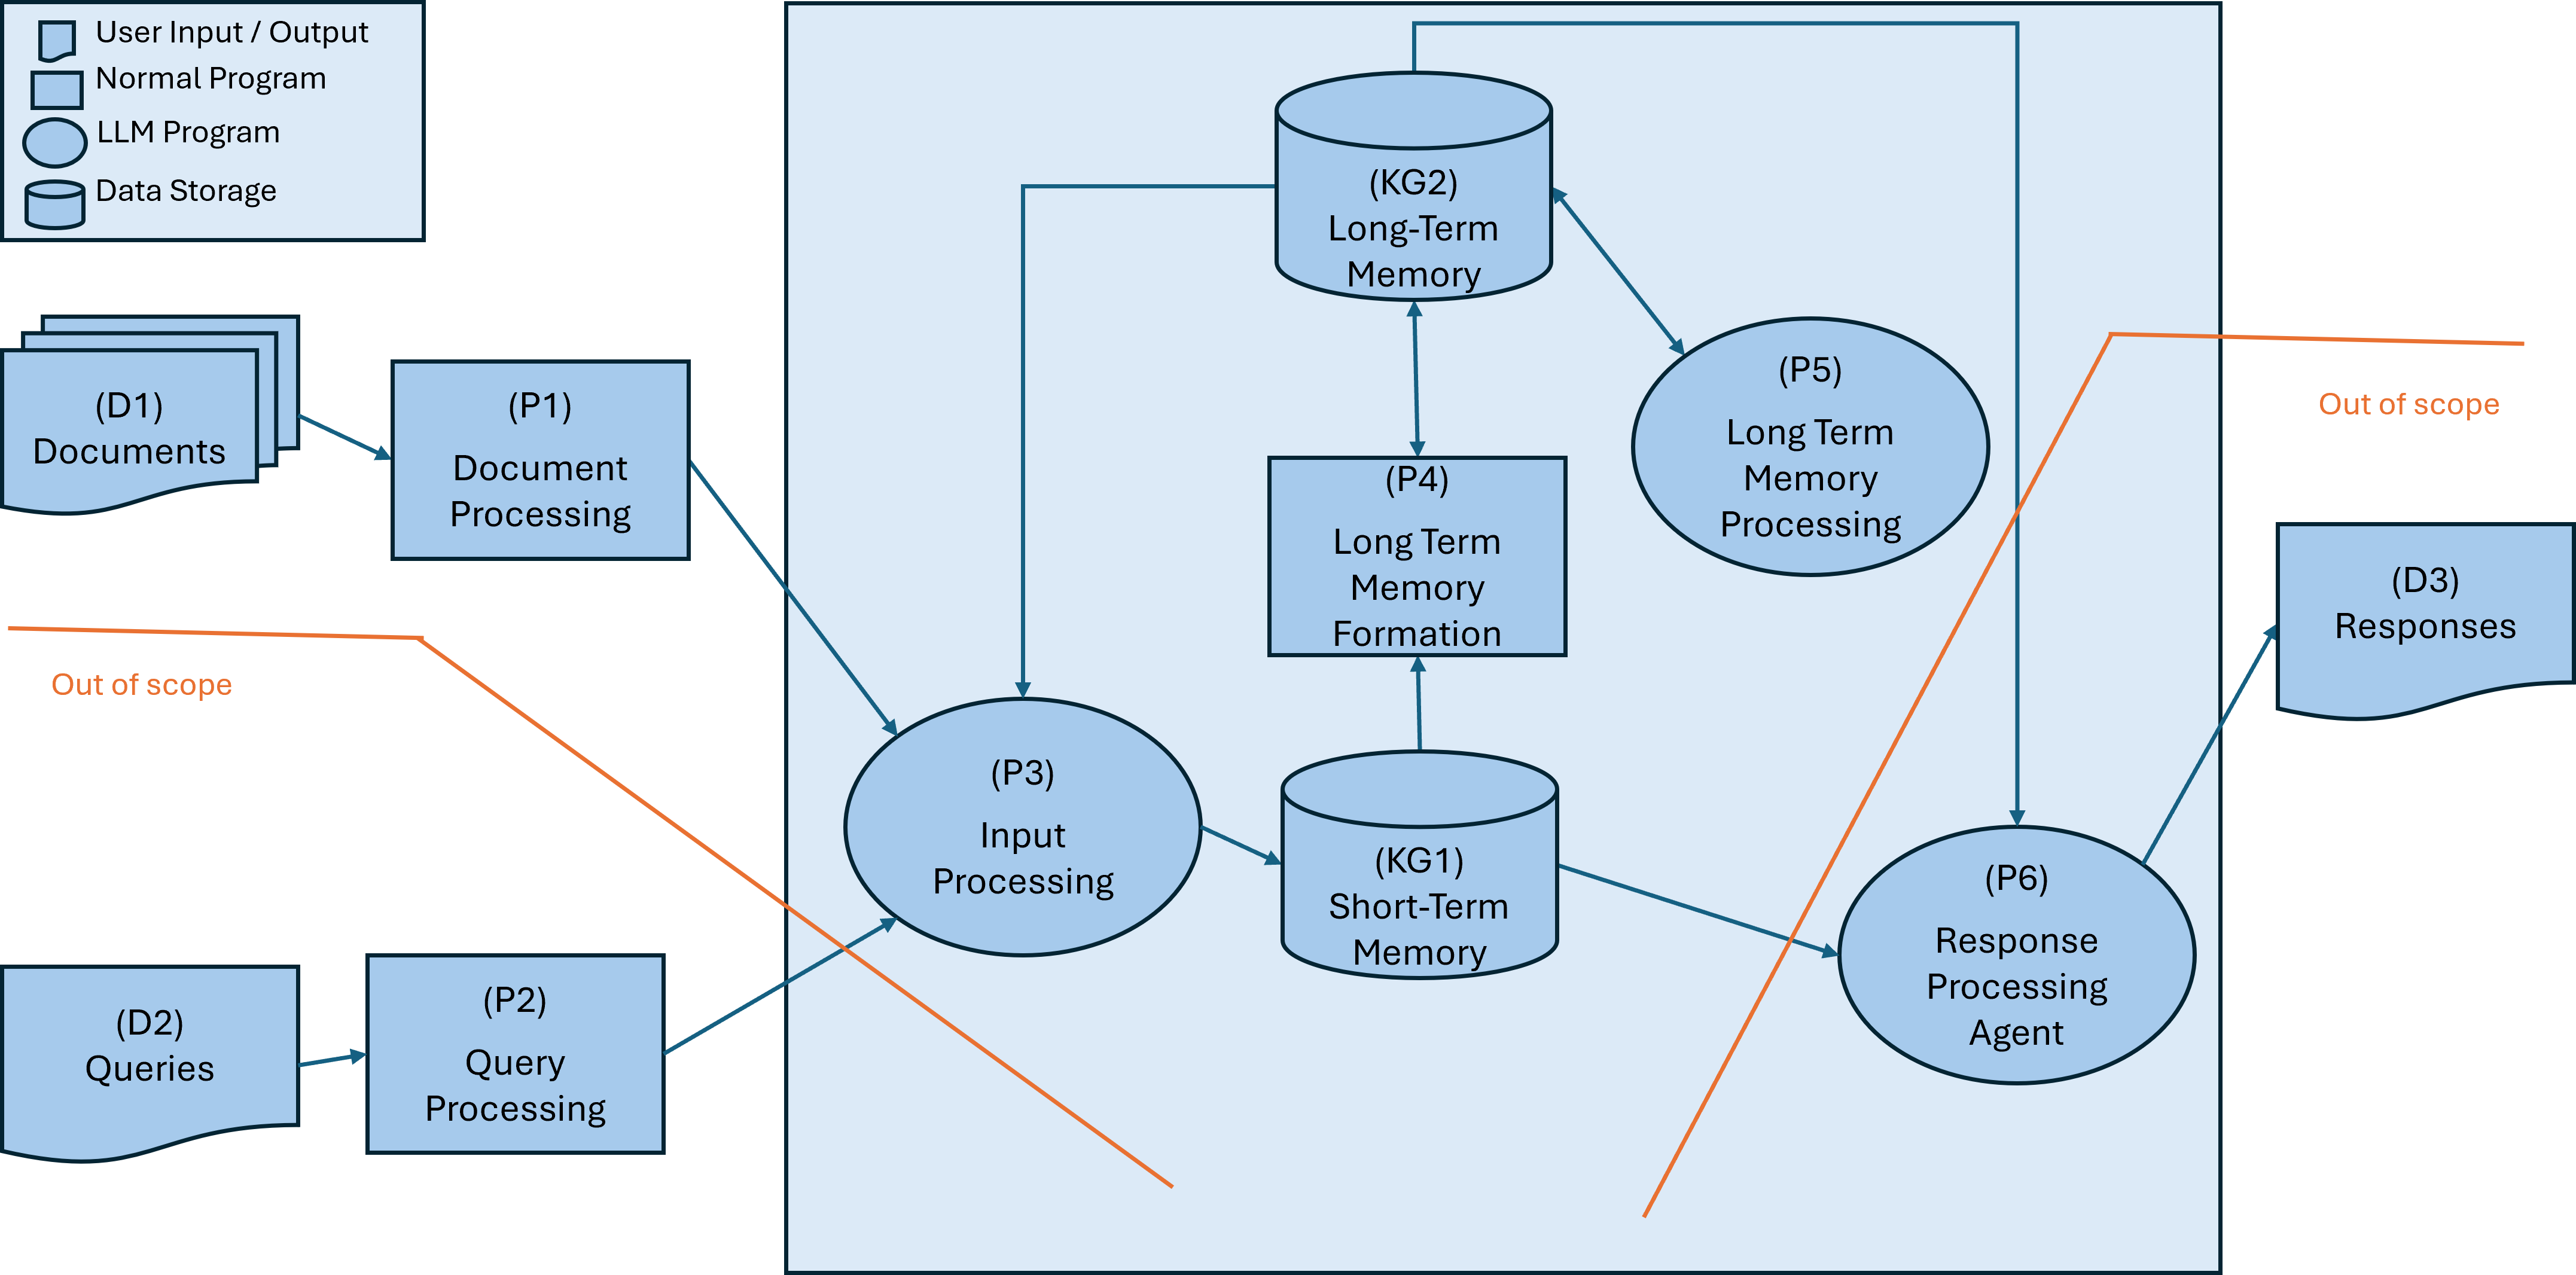
\includegraphics[width=\linewidth]{figures/chap3_fig/Proposed Architecture.png}
    \captionsetup{
        labelfont={bf,it}, 
        textfont=it, 
        justification=centering
    }
    \caption{High-Level Overview of the Document-to-KG Pipeline}
    \label{fig:proposed_architecture}
\end{figure}

\subsubsection{Document Ingestion and Chunking (P1)}
The pipeline begins by ingesting source documents and segmenting them into semantically coherent units, or \textit{chunks}. This chunking process is a critical preprocessing step to overcome the fixed context window of LLMs. A naive split can sever key semantic links; therefore, this component implements and evaluates several intelligent strategies, including fixed-size token windows, paragraph-based segmentation, and overlapping chunks. For hierarchically structured legal documents, a structure-aware strategy leverages the heading styles in DOCX files to ensure chunks do not violate logical boundaries (e.g., articles, sections). Each chunk is meticulously annotated with location metadata (e.g., page, section number) to guarantee end-to-end traceability.

\subsubsection{LLM-Based Information Extraction (P3)}
This component serves as the core information extraction engine. For each text chunk, a carefully engineered prompt instructs an LLM to perform two coordinated tasks: Named Entity Recognition (NER) and Relation Extraction (RE). The model identifies entities corresponding to a predefined legal ontology (e.g., \texttt{Ordinance}, \texttt{DefinedTerm}, \texttt{ZoningDistrict}) and the semantic relationships between them (e.g., \texttt{AMENDS}, \texttt{DEFINES}, \texttt{PERMITS\_IN}). To ensure structured, reliable output, the LLM’s generation is constrained to a predefined JSON schema. The result for each chunk is a self-contained KG fragment, a design that enables parallel processing for enhanced throughput.

\subsubsection{Short-Term Memory (STM): Batch Aggregation (KG1)}
As KG fragments are generated, they are temporarily held in the Short-Term Memory (STM), an in-memory buffer. The STM functions as an efficient staging area, accumulating fragments until a predefined batch size is reached (the "STM fullness threshold" hyperparameter). This batching strategy optimizes performance by reducing the I/O overhead associated with numerous small writes to the persistent database. It also creates an opportunity for low-cost, preliminary consolidation operations before committing the data to long-term storage.

\subsubsection{LTM Ingestion and Entity Resolution (P4 \& KG2)}
Once the STM reaches capacity, the Long-Term Memory (LTM) Ingestion process is triggered. This blocking operation transfers the batch of KG fragments from the STM into the persistent graph database, which constitutes the LTM. The LTM is implemented in Neo4j, a database optimized for highly interconnected data. A crucial step in this process is \textit{entity resolution}, which de-duplicates nodes by merging new entities with existing ones based on unique identifiers or high lexical similarity. For example, multiple mentions of ``Ordinance 2024-05'' are resolved into a single canonical node. This ensures the global KG remains consistent and serves as the definitive, structured representation of the source documents.

\subsubsection{Asynchronous KG Refinement and Enrichment (P5)}
The final stage is an asynchronous engine that performs computationally intensive refinement operations to enhance the global KG's semantic richness. This process operates iteratively on small, random subsets of the graph, allowing the KG to improve gradually without blocking ingestion or requiring complete reprocessing. This stage is triggered only when the primary ingestion pipeline is idle. Key operations include:
\begin{itemize}
    \item \textbf{Ontological Classification:} Formalizing type hierarchies by asserting \texttt{ISA} relationships (e.g., "Ordinance\_123" \texttt{ISA} "Ordinance"), essential for semantic reasoning \parencite{RefWorks:RefID:135-noy2001ontology, RefWorks:RefID:78-minsky1974framework}.
    \item \textbf{Meronymic Relationship Modeling:} Establishing the document's structure within the graph by adding part-whole (\texttt{PARTOF}) relationships (e.g., "Section\_3.B" \texttt{PARTOF} "Article\_III").
    \item \textbf{Type System Refinement:} Identifying and merging semantically equivalent entity types (e.g., consolidating "Regulation" and "Rule") by calculating the similarity of their LLM-generated embeddings \parencite{RefWorks:RefID:167-gardazi2025bert}.
    \item \textbf{Ontology Organization:} Structuring entity types into a coherent subsumption hierarchy using a combination of LLM-based classification and domain heuristics \parencite{RefWorks:RefID:6-2022knowledge}.
    \item \textbf{Instance Type Correction:} Re-classifying entity instances based on new evidence or a more appropriate type within the evolving ontology.
\end{itemize}
This two-tiered memory architecture effectively decouples initial data aggregation from deeper semantic enrichment, creating a robust and scalable framework for KG construction.

\section{Document Processing Workflow}
The journey of a single document through the system is a multi-stage process designed to incrementally build and refine a knowledge graph (KG). This workflow is illustrated in the sequence of diagrams from \cref{fig:chunk_1_processing} to \cref{fig:Long_Term_Memory_processing}. Each figure captures a snapshot of the system's state, showing how data is transformed at each step.

The process begins with the Document Processing stage, where an incoming document is deconstructed into a series of smaller, manageable chunks. These chunks are then processed sequentially. As shown in \cref{fig:chunk_1_processing}, the first chunk is passed to the Input Processor. This component analyzes the text to extract key entities and their relationships, generating a KG fragment. This initial fragment is then stored in the Short-Term Memory (STM), which, as the diagram illustrates, was empty prior to this operation.

\begin{figure}[htp]
    \centering
    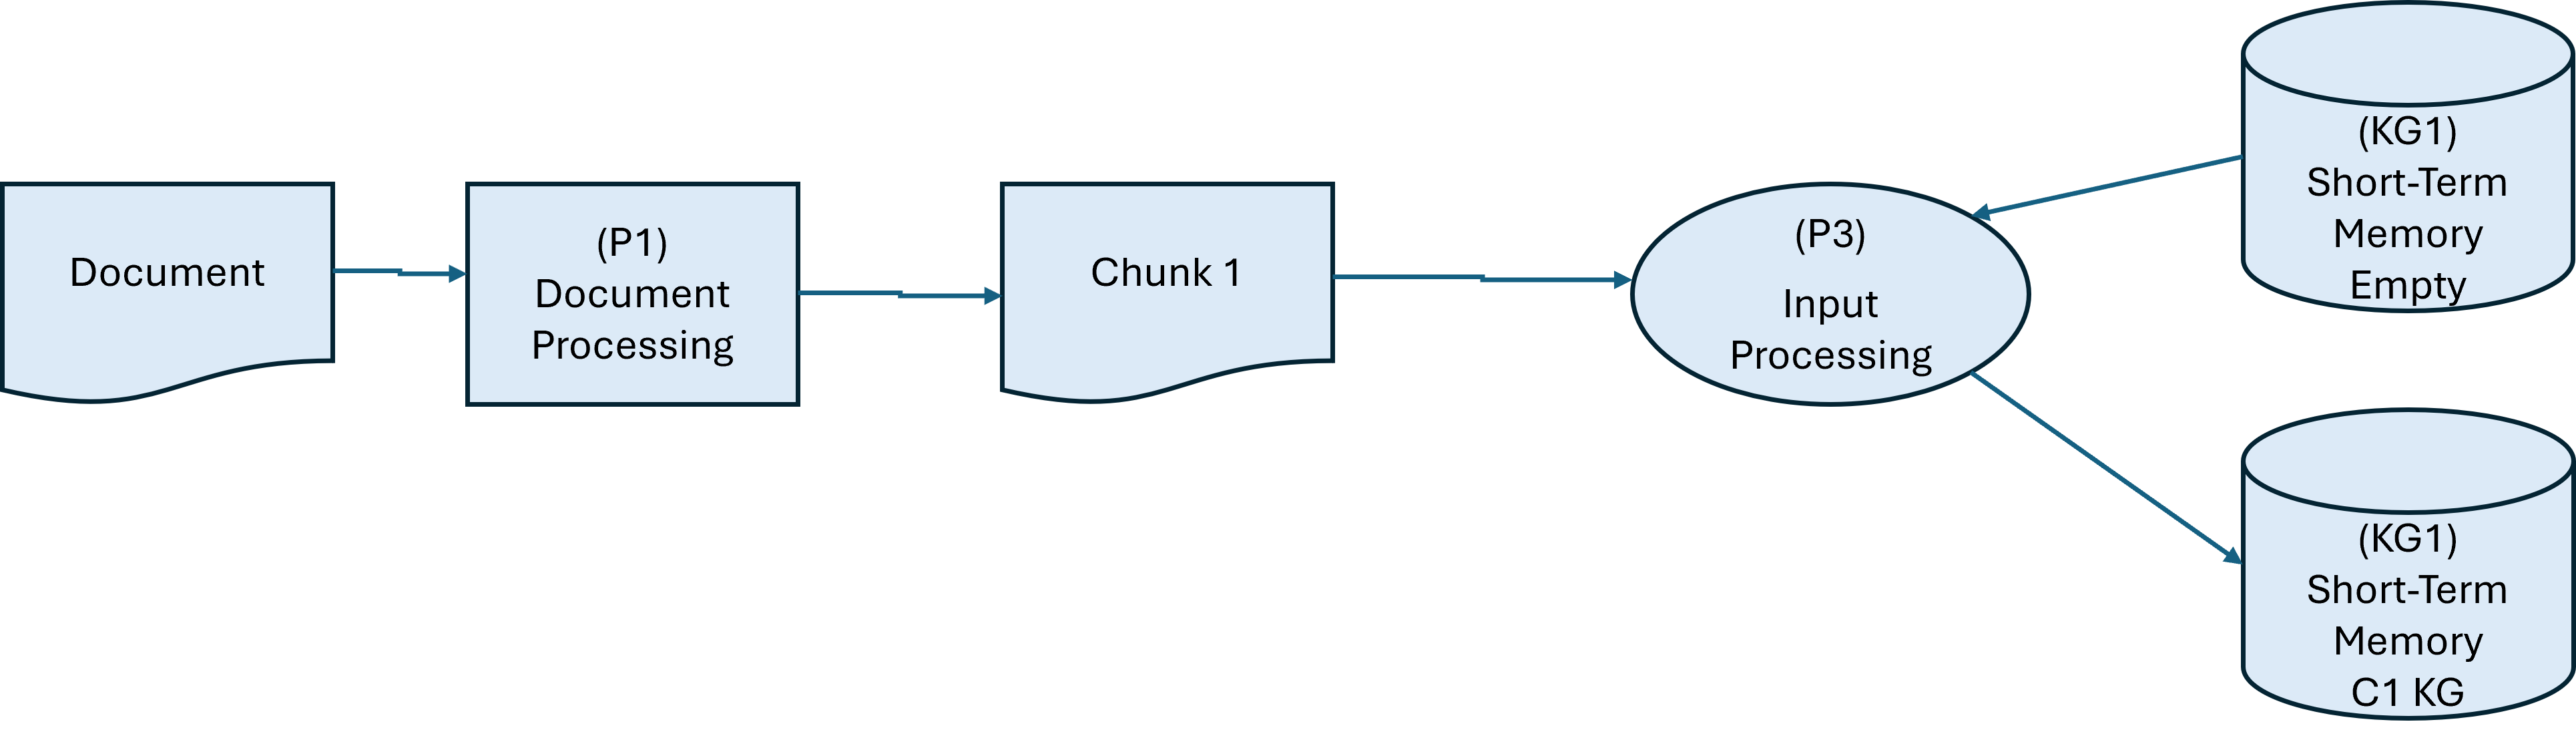
\includegraphics[width=\linewidth]{figures/chap3_fig/Chunk 1 Processing.png}
    \captionsetup{
        labelfont={bf,it},
        textfont=it,
        justification=centering
    }
    \caption{Chunk 1 Processing}
    \label{fig:chunk_1_processing}
\end{figure}

Following the successful processing of the first chunk, the system proceeds to the next one. \cref{fig:chunk_2_processing} depicts this subsequent step. The Input Processor analyzes "Chunk 2" and generates a new KG fragment. This new fragment is then added to the Short-Term Memory. At this stage, the STM contains the distinct knowledge graphs from both the first and second chunks. While basic duplicate detection may occur, the primary goal is rapid ingestion, so the STM accumulates these fragments as largely separate graphs.

\begin{figure}[htp]
    \centering
    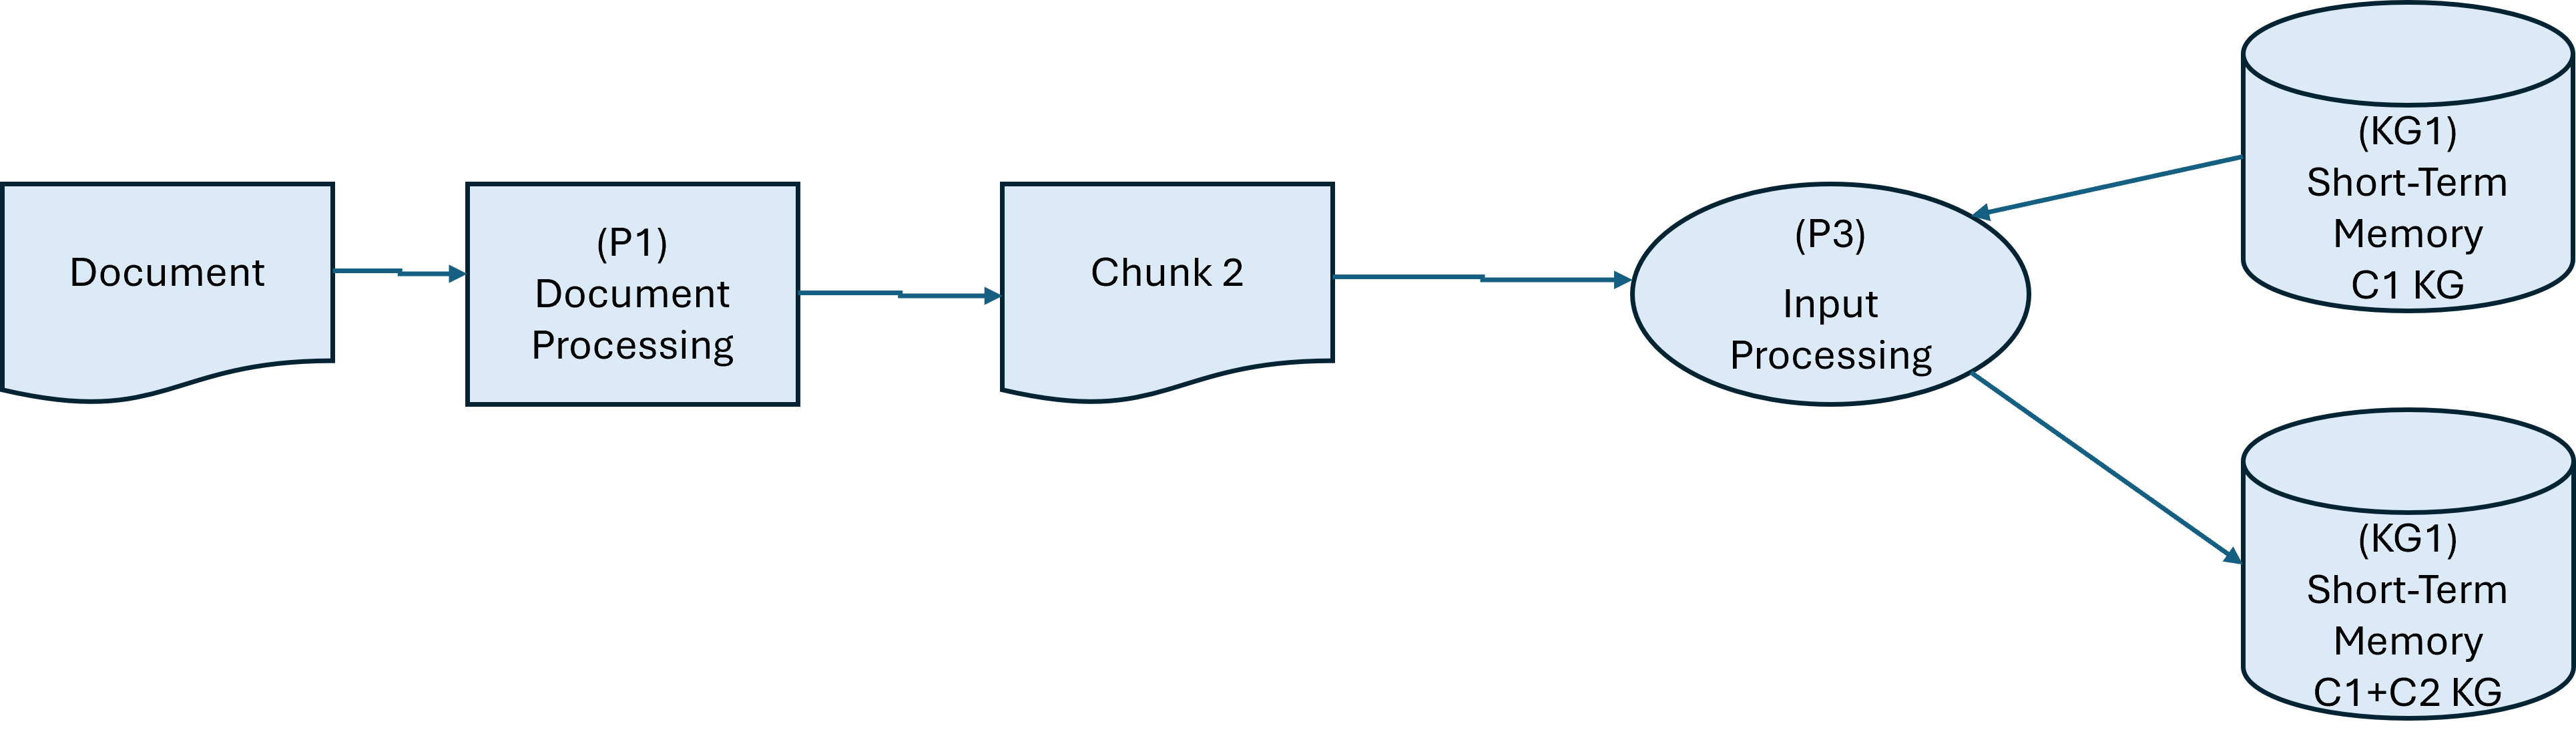
\includegraphics[width=\linewidth]{figures/chap3_fig/Chunk 2 Processing.png}
    \captionsetup{
        labelfont={bf,it},
        textfont=it,
        justification=centering
    }
    \caption{Chunk 2 Processing}
    \label{fig:chunk_2_processing}
\end{figure}

This process of chunk-by-chunk analysis continues until the STM reaches its designated capacity or the document processing is complete. At this point, the LTM Formation process is triggered, as illustrated in \cref{fig:Full_STM_processing}. The entire collection of KG fragments held in the STM is transferred to be consolidated. This consolidation phase merges the individual fragments, resolves redundancies, and integrates the new information into the persistent Long-Term Memory (LTM). Once the transfer and consolidation are complete, the STM is cleared, making it ready to process the next chunk or document.

\begin{figure}[htp]
    \centering
    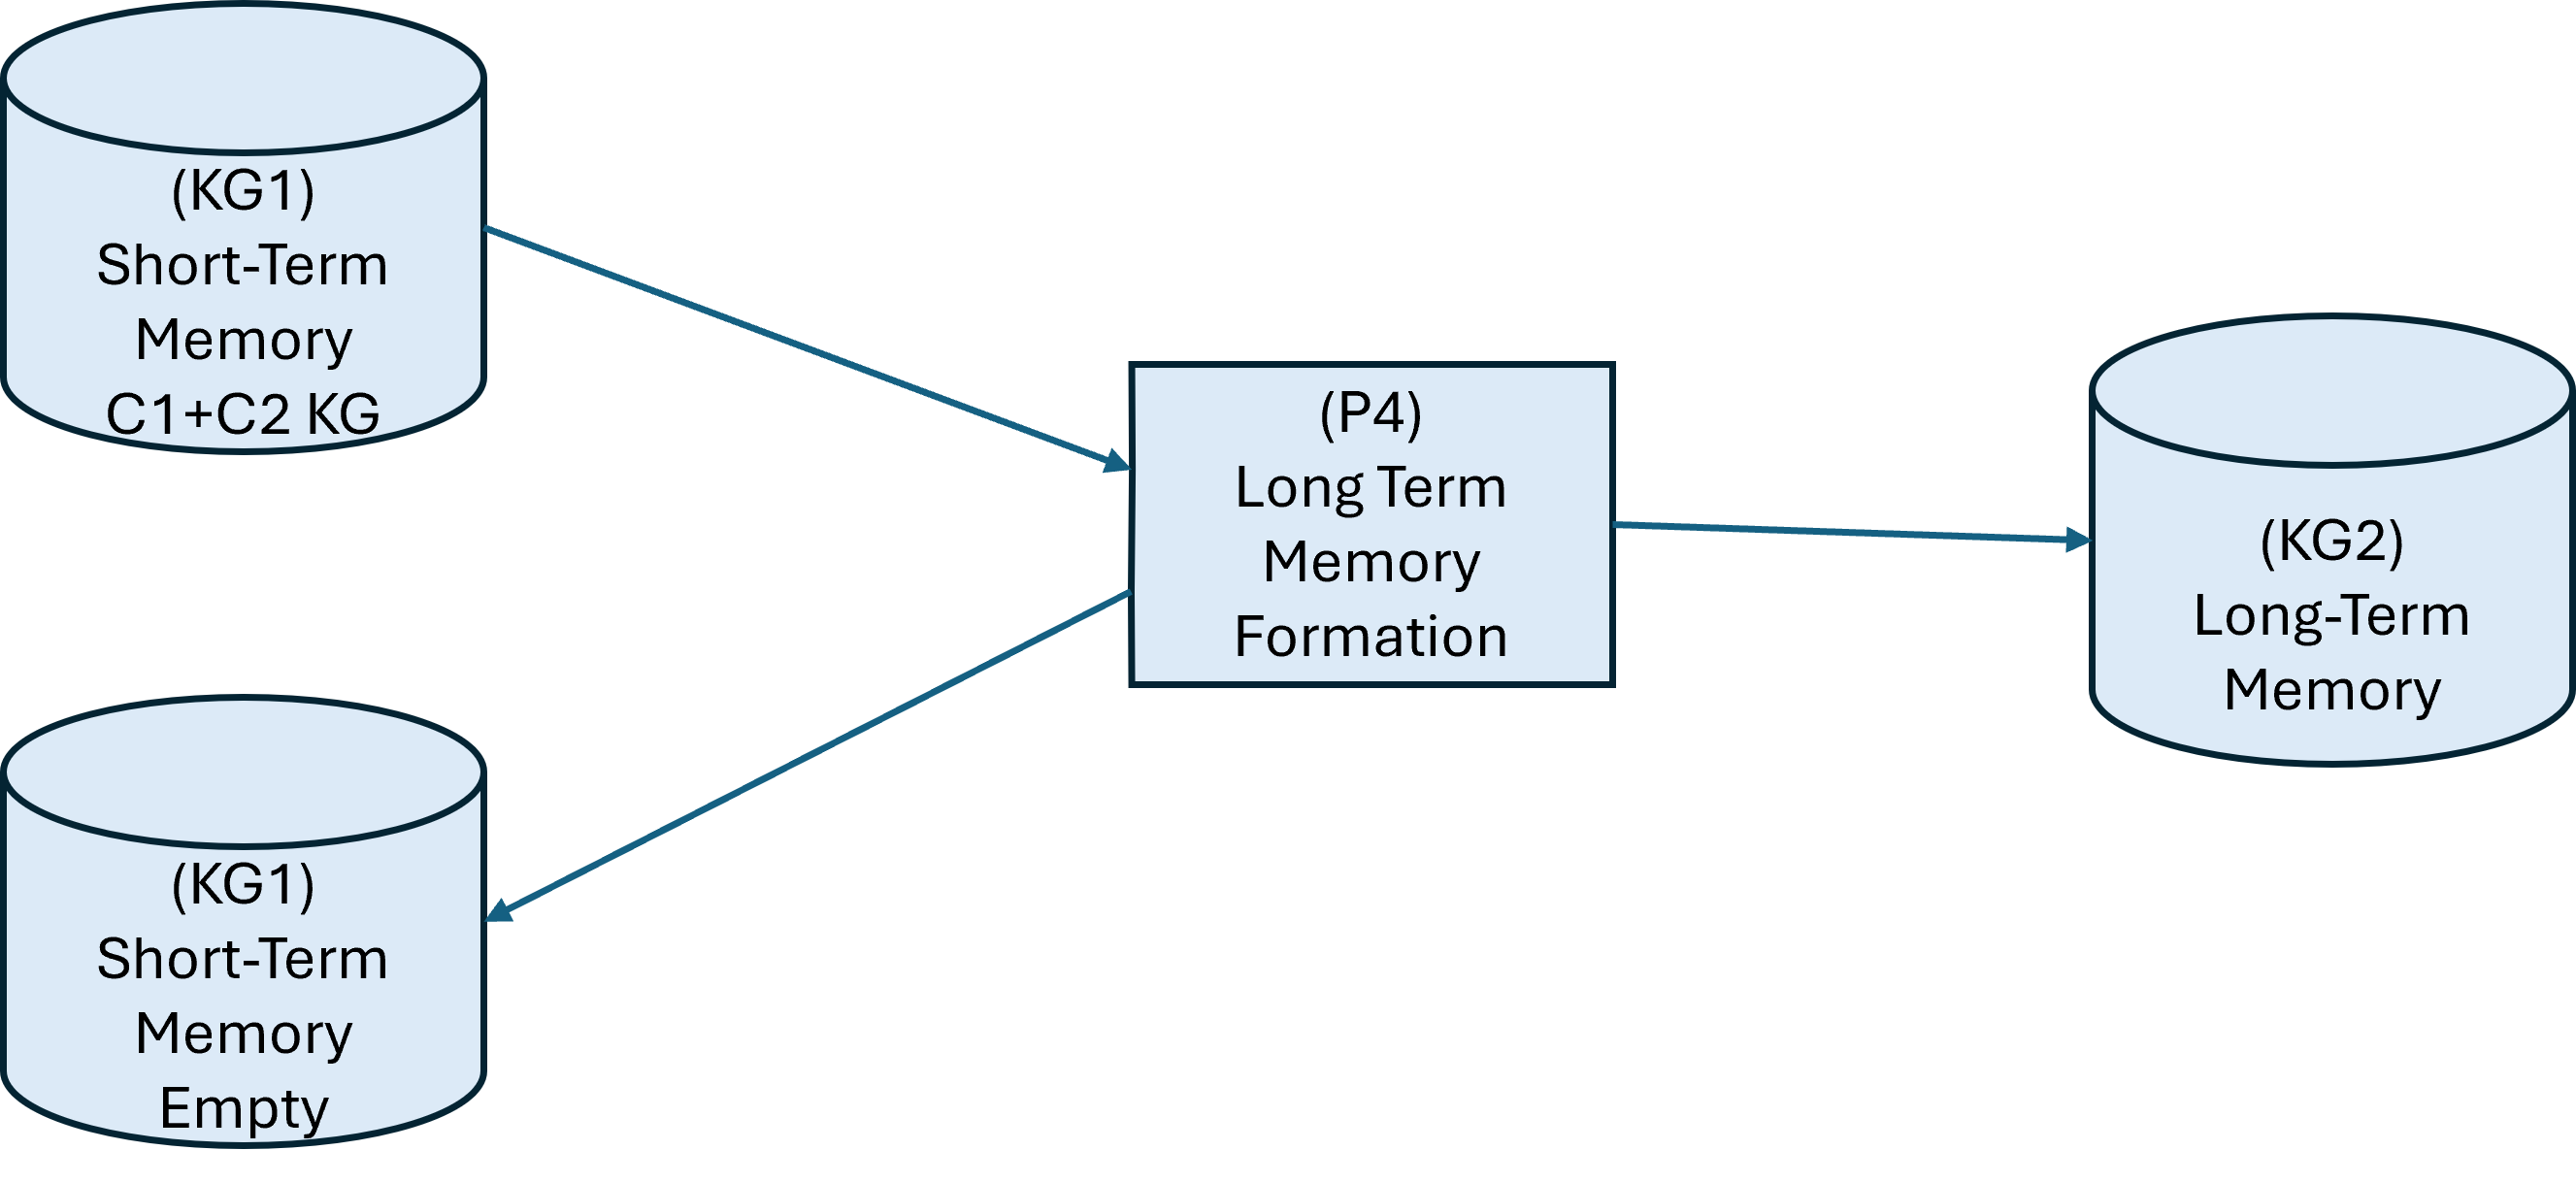
\includegraphics[width=\linewidth]{figures/chap3_fig/Full Short Term Memory.png}
    \captionsetup{
        labelfont={bf,it},
        textfont=it,
        justification=centering
    }
    \caption{Full Short Term Memory Processing}
    \label{fig:Full_STM_processing}
\end{figure}

Finally, the LTM is not a static repository. As depicted in \cref{fig:Long_Term_Memory_processing}, an asynchronous LTM Processing engine operates continuously in the background. This engine performs computationally intensive refinement tasks on the global KG stored in the LTM. These tasks include advanced entity disambiguation, inference of new relationships, and overall structural optimization of the graph. This continuous refinement ensures that the knowledge base becomes more accurate, coherent, and semantically rich over time.

\begin{figure}[htp]
    \centering
    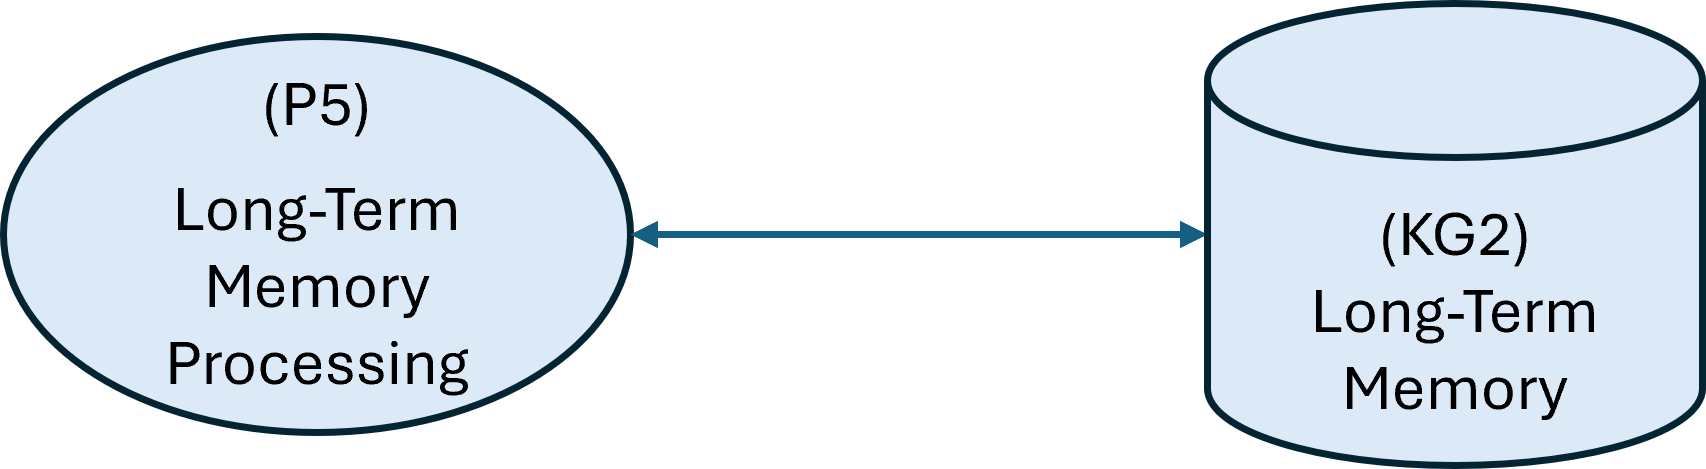
\includegraphics[width=\linewidth]{figures/chap3_fig/Long Term Memory Processing.png}
    \captionsetup{
        labelfont={bf,it},
        textfont=it,
        justification=centering
    }
    \caption{Long Term Memory Processing}
    \label{fig:Long_Term_Memory_processing}
\end{figure}

In summary, this entire workflow represents a cyclical and scalable approach to knowledge extraction and management. The division between a fast, transient Short-Term Memory and a persistent, refined Long-Term Memory allows the system to process information efficiently without sacrificing the quality and coherence of the final knowledge graph. The initial, rapid ingestion into STM ensures that incoming data is captured without delay, while the subsequent consolidation and asynchronous refinement processes guarantee that the LTM evolves into a comprehensive and accurate representation of the knowledge contained within the source documents. This dual-memory architecture is key to balancing the demands of real-time processing with the need for deep, semantic integration.

\section{Knowledge Graph Data Model for Legal Text Analysis}
A robust data model is foundational to the development of a Knowledge Graph (KG) capable of representing complex legal corpora and facilitating sophisticated analytical queries. This section details the proposed ontological framework for a Neo4j-based Legal TTP (LTM), designed to capture the semantic structure of municipal legal codes. The model's schema is engineered for both representational fidelity to the source text and the computational efficiency required for automated consistency and completeness validation.

\subsection{Ontological Framework: Node Schema}
The core entities within the legal documents are modeled as nodes, each assigned one or more labels that denote its classification. Nodes possess a set of properties that store their specific attributes, extracted directly from the text. The primary node labels and their associated properties are enumerated in \cref{tab:node_schema}.

\begin{table}[htbp]
\centering
\captionsetup{
    labelfont={bf,it}, 
    textfont=it, 
    justification=centering
}
\caption{Node Schema and Property Definitions.}
\label{tab:node_schema}
\begin{tabularx}{\textwidth}{@{} >{\raggedright}p{0.22\textwidth} >{\raggedright}p{0.45\textwidth} >{\raggedright\arraybackslash}p{0.33\textwidth} @{}}
\toprule
\textbf{Node Label} & \textbf{Description} & \textbf{Key Properties} \\ 
\midrule
\texttt{DocumentSection} & A structural component of the legal code, such as a chapter, article, or section, serving as a container for legal rules. & \texttt{id}, \texttt{title}, \texttt{textContent}, \texttt{sourceLocation} \\ 
\addlinespace
\texttt{DefinedTerm} & An explicit definition of a specialized term provided within the legal text. & \texttt{term}, \texttt{definitionText}, \texttt{sourceLocation} \\ 
\addlinespace
\texttt{Ordinance} & A formal legislative act, such as a law or an amendment, that creates, modifies, or repeals portions of the code. & \texttt{ordinanceNumber}, \texttt{enactmentDate}, \texttt{title} \\ 
\addlinespace
\texttt{ZoningDistrict} & A geographically delineated area subject to a specific set of land-use regulations. & \texttt{districtName}, \texttt{districtCode} \\ 
\addlinespace
\texttt{PermittedUse} & A specific activity, function, or land use that is legally sanctioned within a given zoning district, potentially under certain conditions. & \texttt{useName}, \texttt{conditions} \\ 
\addlinespace
\texttt{Obligation} & A deontic expression imposing a legal duty or permission on a specific actor (e.g., a requirement to obtain a permit). & \texttt{actor}, \texttt{action}, \texttt{modality} (e.g., MUST, MAY, NOT\_PERMITTED) \\ 
\addlinespace
\texttt{Reference} & A citation pointing to another legal provision, either internal or external to the current code. & \texttt{targetIdentifier}, \texttt{referenceType} (e.g., INTERNAL, EXTERNAL), \texttt{sourceText} \\ 
\bottomrule
\end{tabularx}
\end{table}

\subsection{Semantic Relations: Edge Schema}
The semantic connections and interactions between nodes are represented by directed, typed edges, formally known as relationships. The type of each relationship specifies the precise nature of the connection between the source and target nodes. \Cref{tab:relationship_schema} presents the defined relationship types.

\begin{table}[htbp]
\centering
\captionsetup{
    labelfont={bf,it}, 
    textfont=it, 
    justification=centering
}
\caption{Relationship Schema and Semantic Descriptions.}
\label{tab:relationship_schema}
\begin{tabularx}{\textwidth}{@{} >{\raggedright}p{0.2\textwidth} >{\raggedright}X L{0.15\textwidth} @{}}
\toprule
\textbf{Relationship Type} & \textbf{Description (Source \(\rightarrow\) Target)} & \textbf{Properties} \\
\midrule
\texttt{CONTAINS} & \texttt{DocumentSection} \(\rightarrow\) \texttt{DocumentSection}. Models the hierarchical structure of the code (e.g., a chapter contains a section). & -- \\
\addlinespace
\texttt{DEFINES} & \texttt{DocumentSection} \(\rightarrow\) \texttt{DefinedTerm}. Links a section of text to a term it formally defines. & -- \\
\addlinespace
\texttt{AMENDS} & \texttt{Ordinance} \(\rightarrow\) \texttt{DocumentSection}. Signifies that a law modifies a specific part of the code. & \texttt{effectiveDate} \\
\addlinespace
\texttt{CITES} & \texttt{DocumentSection} \(\rightarrow\) \texttt{Reference}. Indicates that a section of the code makes a citation. & -- \\
\addlinespace
\texttt{PERMITS} & \texttt{ZoningDistrict} \(\rightarrow\) \texttt{PermittedUse}. Specifies that a land use is allowed within a particular district. & -- \\
\addlinespace
\texttt{IMPOSES} & \texttt{DocumentSection} \(\rightarrow\) \texttt{Obligation}. Connects a legal rule to the specific duty or permission it creates. & -- \\
\addlinespace
\texttt{USES\_TERM} & \texttt{DocumentSection} \(\rightarrow\) \texttt{DefinedTerm}. Denotes the usage of a previously defined term within a section. & -- \\
\bottomrule
\end{tabularx}
\end{table}

\subsection{Model Application: Inconsistency Detection}
This ontological structure provides the necessary foundation for executing complex graph-based queries to automatically identify potential inconsistencies within the legal corpus. For instance, a critical validation is to detect the use of terms that have not been formally defined. This scenario corresponds to a \texttt{DocumentSection} node that has an outgoing \texttt{USES\_TERM} relationship to a \texttt{DefinedTerm} node, but where that \texttt{DefinedTerm} node lacks an incoming \texttt{DEFINES} relationship from any \texttt{DocumentSection}.

Such a query can be expressed declaratively using a graph pattern matching language like Cypher. The pattern to identify an undefined term (\texttt{dt}) being used in a section (\texttt{ds}) would be:
\begin{verbatim}
MATCH (ds:DocumentSection)-[:USES_TERM]->(dt:DefinedTerm)
WHERE NOT EXISTS ((:DocumentSection)-[:DEFINES]->(dt))
RETURN ds.id, dt.term
\end{verbatim}
The execution of this and similar queries across the KG enables a systematic and scalable methodology for auditing the logical coherence of the legal code, thereby demonstrating the analytical utility of the proposed data model.

\section{Dataset and Pre-processing}
This research requires a corpus of large, complex documents to rigorously test the proposed methodology. The dataset must be readily accessible and available in a format that permits modification for experimental purposes, such as error injection tests. 

\subsection{Dataset Selection and Rationale}
The primary dataset comprises the codified ordinances of various townships within the Commonwealth of Pennsylvania. This choice is predicated on several factors aligned with the research objectives. These documents are voluminous and linguistically complex, presenting a suitable challenge. Their public availability simplifies acquisition and supports open research principles. Legal codes contain rich interrelationships—such as cross-references, definitions, and amendments—that are well-suited for KG representation. The dataset directly addresses the problem of inconsistency in municipal laws identified in Chapter 1 \parencite{RefWorks:RefID:144-curley2024municipal, RefWorks:RefID:145-rau2024municipal}. Finally, the researcher’s domain familiarity aids in the interpretation of legal nuances.

\subsection{Data Acquisition and Pre-processing}
The township law documents will be acquired from online public sources, primarily the legal code aggregator eCode360 \parencite{RefWorks:RefID:146-sanders2024municipal}. The documents will be obtained in DOCX format, which is preferred over PDF because it preserves structural information (e.g., heading styles, lists, tables) that is advantageous for developing semantically aware chunking strategies. 

An initial Exploratory Data Analysis (EDA) will be conducted on a representative sample of 5-10 municipal codes. This EDA will serve to:
\begin{itemize}
    \item Characterize the typical document structure, length, and complexity.
    \item Identify the most common entity types and relationship patterns.
    \item Analyze linguistic features, such as the prevalence of legal jargon and complex sentence structures.
\end{itemize}
The findings from this EDA will directly inform the refinement of the KG data model, the design of chunking strategies, and the formulation of effective LLM prompts. Following the EDA, the pre-processing pipeline will be finalized. It will involve extracting the core textual content, removing irrelevant artifacts (e.g., headers, footers, page numbers), and normalizing the text (e.g., handling special characters, standardizing case) to create a clean corpus for processing.

\section{Hyperparameters}
The performance and behavior of the pipeline are governed by several critical hyperparameters. The systematic tuning of these parameters is essential for optimizing the system for accuracy and efficiency. The experimental plan involves varying these parameters and evaluating their impact using the metrics defined in Section 3.7. A summary of the parameters to be tuned is presented in \cref{tab:hyperparameter_exp_design}.

The foundational choice is the \textbf{LLM Model}. Various models, including those from the Google Gemini, OpenAI GPT, and Anthropic Claude families, will be evaluated to find the optimal balance of extraction accuracy, adherence to structured output formats, and operational cost within the specialized legal domain. The \textbf{LLM Temperature} will be tuned within a low range (e.g., 0.0 to 0.7) to favor deterministic, factual extraction over creative but potentially inaccurate outputs, with the goal of minimizing hallucinations \parencite{RefWorks:RefID:96-rzepka2023expert}. Furthermore, \textbf{Prompt Design} will be an iterative process of refinement to improve clarity, specificity, and the inclusion of few-shot examples to better guide the model's NER and RE tasks.

\textbf{Document Chunking} strategies are vital for managing the context window limitations of LLMs \parencite{RefWorks:RefID:115-ratner2022parallel}. Different strategies will be tested to determine which best preserves semantic context across chunk boundaries \parencite{RefWorks:RefID:104-qu2024semantic}. For paragraph-based chunking, the number of \textbf{Paragraphs per Chunk} will be varied to find the ideal semantic unit size. For overlapping strategies, the \textbf{Overlap Percentage} will be adjusted to manage the trade-off between context continuity and redundant processing. The absolute \textbf{Chunk Size} in tokens will also be tuned to maximize the local context available to the selected LLM.

Finally, \textbf{Processing} parameters control the asynchronous consolidation and refinement of the KG. The \textbf{STM Fullness Threshold} dictates how many KG fragments are batched before being moved to the LTM, balancing data freshness with processing overhead. The \textbf{LTM Formation Batch Size} controls the resource intensity of these consolidation cycles. Similarly, the \textbf{LTM Processing Batch Size} determines the number of nodes to be refined in each asynchronous cycle, balancing processing depth with computational cost. The \textbf{Frequency of LTM Processing} controls the overall rate of iterative refinement of the global KG.
\begin{table}[htbp]
\centering
\captionsetup{
    labelfont={bf,it}, 
    textfont=it,  
    justification=centering
    }
\caption{Hyperparameter Categories and Specific Parameters.}
\label{tab:hyperparameter_exp_design}
% Use tabularx and set its width to the width of the text block
\begin{tabularx}{\textwidth}{@{} lX @{}} 
\toprule
\textbf{Category} & \textbf{Parameter} \\
\midrule
\addlinespace
\textbf{LLM Used} & LLM Model \\
& LLM Temperature \\
& Prompt Design \\
\addlinespace
\hline
\addlinespace
\textbf{Document Chunking} & Strategy \\
& Paragraphs per Chunk \\
& Overlap Percentage \\
& Chunk Size (Tokens) \\
\addlinespace
\hline
\addlinespace
\textbf{Processing} & STM Fullness Threshold (Number of KGs) \\
& LTM Formation Batch Size \\
& LTM Processing Batch Size (Number of Nodes) \\
& Frequency of LTM Processing \\
\addlinespace
\bottomrule
\end{tabularx}
\end{table}

\section{System Implementation and Environment}
\label{sec:technical_environment}
\label{sec:methodology_env}
The methodology will be implemented using a standard, robust set of tools for AI and NLP research, ensuring reproducibility and leveraging the strengths of the current software ecosystem.
\begin{itemize}
    \item \textbf{Core Language:} Python (version 3.8+) will be the primary programming language due to its extensive libraries for data science, NLP, and API integration.
    \item \textbf{Development Environment:} Google Colaboratory will be used for development and experimentation, providing access to necessary computational resources, including GPUs for potentially hosting smaller, open-source LLMs or for embedding generation.
    \item \textbf{LLM Interaction:} The LangChain framework \parencite{RefWorks:RefID:101-zhao2023survey} will be utilized to manage interactions with various LLM APIs. LangChain provides useful abstractions for prompt management, output parsing, and chaining together different components of the pipeline.
    \item \textbf{Graph Database:} The Long-Term Memory (LTM) will be implemented using Neo4j (version 5.x), a native graph database. Its Cypher query language is highly expressive and well-suited for the complex pattern matching required for KG analysis and integrity checking \parencite{RefWorks:RefID:111-kumar2013querying}.
    \item \textbf{Document Parsing:} The `python-docx` library will be used to parse the input DOCX files, allowing for the extraction of both textual content and structural information like headings.
    \item \textbf{Version Control:} All code and configuration files will be managed using Git and hosted on GitHub. This practice ensures version control, facilitates collaboration, and guarantees the reproducibility of the research.
\end{itemize}

\section{Evaluation Measurements}
Evaluating the quality of the generated KG is a non-trivial task, primarily due to the difficulty of establishing a "gold standard" ground truth for large, complex legal documents \parencite{RefWorks:RefID:76-dhani2021similar}. Therefore, the evaluation strategy is multi-faceted, combining quantitative, qualitative, intrinsic, and extrinsic measures to provide a holistic assessment of the KG's fidelity and utility. This strategy is summarized in Table \cref{tab:measurement_metrics_summary}.

\subsection{Knowledge Graph Fit Assessment}
This area of evaluation addresses how well the generated KG represents the source documents.
\begin{itemize}
    \item \textbf{Entity/Relation Extraction Quality:} The core extraction quality will be measured using standard metrics of Precision, Recall, and F1-score. A sample of 100-200 document chunks will be manually annotated to create a ground-truth dataset. The system's output on this sample will be compared against the manual annotations. A target F1-score above 0.8 is set for key legal entity and relation types.
    \item \textbf{Content Coverage and Plausibility (Expert Review):} A qualitative review will be conducted by one or more individuals with legal domain expertise (ideally the researcher and a peer). They will inspect randomly selected subgraphs of the KG and compare them against the corresponding source text. The goal is to achieve high inter-rater agreement that key legal concepts are present, accurately represented, and logically connected.
    \item \textbf{Traceability:} This will be measured by randomly sampling 100 nodes and relationships from the KG and verifying that their `source\_location` property correctly links back to the precise text in the source document from which they were extracted. The target for this metric is over 95\% accuracy to ensure verifiability.
    \item \textbf{KG Structural Integrity:} This will be analyzed by examining graph-level statistics before and after LTM Processing. Metrics will include node and edge distributions, graph density, and connectivity. The goal is to demonstrate that the LTM processing steps lead to a more coherent and well-formed graph structure (e.g., fewer disconnected components, more logical type hierarchies).
\end{itemize}

\subsection{Suitability for Consistency and Completeness (C\&C) Analysis}
This assessment determines if the KG is structured in a way that supports the end goal of C\&C analysis, even though the full implementation of C\&C algorithms is designated as future work.
\begin{itemize}
    \item \textbf{Presence of Requisite Information Types:} A checklist-based evaluation will be performed to ensure that the information types necessary for C\&C checks (e.g., definitions, obligations, cross-references, deadlines) are being successfully extracted and represented in the KG.
    \item \textbf{Queryability for Integrity Patterns:} A set of predefined Cypher queries will be executed against the KG to test for common integrity patterns. Examples include queries to find: (1) terms used in the text but never defined, (2) sections referenced but not present, and (3) conflicting obligations applied to the same entity. The goal is to confirm that the KG structure supports such queries and returns plausible candidates for inconsistencies.
    \item \textbf{KG Schema/Ontology Quality:} The emergent ontology of entity types will be qualitatively assessed for its clarity, coherence, and appropriateness for the legal domain. This ensures the schema is robust enough to support downstream legal C\&C applications.
\end{itemize}

\subsection{Controlled Error Injection Experiment}
To provide a more objective measure of the system's ability to facilitate error detection, a controlled experiment will be conducted. A "gold standard" clean legal document will be seeded with a variety of common legal document errors to create a synthetic ground truth \parencite{RefWorks:RefID:140-mintz2009distant}. A typology of errors to be injected includes:
\begin{itemize}
    \item \textbf{Type 1: Contradictory Definition:} Defining the same term in two different ways in separate sections.
    \item \textbf{Type 2: Undefined Term:} Using a specialized legal term throughout a section without providing an explicit definition.
    \item \textbf{Type 3: Broken Reference:} Including a cross-reference to a section number that does not exist (e.g., "as described in Section 99.9").
    \item \textbf{Type 4: Conflicting Obligation:} Stating in one section that a permit "is required" for an activity and in another that it "is not required" under the same conditions.
    \item \textbf{Type 5: Incomplete Specification:} Mentioning that a fee is required but failing to specify the amount or the calculation method.
\end{itemize}
The primary metric will be the \textbf{Error Detection Rate (EDR)}, defined as the percentage of these injected errors that are identifiable through specific queries on the generated KG. The \textbf{Traceability of Error Indicators} will also be measured to ensure that the KG elements flagging an error can be accurately traced back to the specific erroneous text in the source document.

\begin{table}[htbp]
\centering
\captionsetup{
    labelfont={bf,it}, 
    textfont=it,  
    justification=centering
    }
\caption{Summary of Measurement Metrics.}
\label{tab:measurement_metrics_summary}
% Use tabularx to make the table fit the text width.
% The 'X' column will wrap the long text automatically.
\begin{tabularx}{\textwidth}{@{} lX @{}}
\toprule
\textbf{Category} & \textbf{Metric} \\
\midrule
\addlinespace
\textbf{Knowledge Graph Fit} & Entity/Relation Extraction (Precision, Recall, F1-score) \\
& Content Coverage \& Plausibility \\
& Traceability \\
& KG Structural Integrity \\
\addlinespace
\hline
\addlinespace
\textbf{Suitability for C\&C Analysis} & Presence of Requisite Information Types \\
& Queryability for Integrity Patterns \\
& KG Schema/Ontology Quality \\
\addlinespace
\hline
\addlinespace
\textbf{Error Injection} & Error Detection Rate (EDR) \\
& Traceability of Error Indicators \\
\addlinespace
\bottomrule
\end{tabularx}
\end{table}

\section{Methodological Limitations}
This research acknowledges several limitations. The system's accuracy is dependent on the capabilities of the underlying LLM, which can hallucinate or misinterpret nuanced text \parencite{RefWorks:RefID:101-zhao2023survey}. Document chunking inherently risks losing context that spans across chunks \parencite{RefWorks:RefID:104-qu2024semantic}. KG evaluation involves subjective judgment in the absence of a comprehensive ground truth, and errors in early pipeline stages can propagate \parencite{RefWorks:RefID:121-zhong2024comprehensive}. The scope of this praxis is limited to textual content (excluding complex tables, figures, and formulas), and the system is developed and evaluated on Pennsylvania township laws; performance on other legal document types may vary. Finally, this work focuses on generating a KG *suitable* for C\&C checks; the implementation and evaluation of a fully automated C\&C system is designated as future work \parencite{RefWorks:RefID:10-zowghi2003interplay}.

\section{Ethical Considerations}
The research is guided by several ethical principles. The data consists of public records, and no private or sensitive information is processed. The system is intended as an assistive tool for legal experts, not a replacement for human judgment; the emphasis on traceability mitigates the risk of over-reliance and promotes transparency. The potential for LLMs to perpetuate biases present in their training data is acknowledged, although the narrow domain of legal texts may limit the impact of broader societal biases \parencite{RefWorks:RefID:101-zhao2023survey}. All intellectual property will be handled according to university policy, and the principles of responsible innovation will be followed throughout the research.

\section{Conclusion}
This chapter has presented a detailed, multi-faceted methodology for developing and evaluating an LLM-based system to convert large legal documents into KGs. The objective is to create a robust and verifiable foundation for the future analysis of document consistency and completeness. The approach specifies a modular multi-stage pipeline, a comprehensive data model, a systematic plan for hyperparameter tuning, and a rigorous evaluation strategy that combines quantitative metrics, qualitative reviews, and a controlled error injection experiment. By addressing inherent limitations and adhering to ethical considerations, this methodology provides a structured and defensible plan to investigate the research questions and test the hypotheses set forth in Chapter 1.

\section{Research Questions}
This methodology is designed to address the following research questions:

\textbf{RQ1:} Can an LLM be used to convert a large document into a knowledge graph?

\textbf{RQ2:} Can an LLM be used to process multiple knowledge graphs into a typed cluster of knowledge graphs.

\textbf{RQ3:} Can a typed cluster of knowledge graphs be used to check the source document for consistency and completeness?

\section{Research Hypotheses}
The research will test the following hypotheses:

\textbf{H1:} An LLM can be used to convert a large document into a knowledge graph.

\textbf{H2:} An LLM can be used to process multiple knowledge graphs into a typed cluster of knowledge graphs.

\textbf{H3:} A typed cluster of knowledge graphs can be used to check the source document for consistency and completeness.
